\documentclass[a4paper,11pt]{article}

\usepackage[top=1.5in, bottom=1.5in, left=0.8in, right=0.8in]{geometry}
\usepackage[utf8]{inputenc}
\usepackage[T1]{fontenc}
\usepackage[english,polish]{babel}
\usepackage{indentfirst}
\usepackage{multirow}
\usepackage{graphicx}
\usepackage{subfig}
\usepackage[all]{nowidow} 
\usepackage{titletoc}
\usepackage{listings}
\usepackage{color}
\usepackage{relsize}
\usepackage{chngcntr}
\usepackage{longtable}
\usepackage{float}
\usepackage[table]{xcolor} 
\usepackage{rotating}
\clubpenalty10000
\widowpenalty10000
\counterwithin{figure}{section}
\counterwithin{table}{section}

\linespread{1.3}
\setcounter{secnumdepth}{5}
\setcounter{tocdepth}{5}
\begin{document}
% definicje 
\makeatletter
\newcommand{\linia}{\noindent\rule{\linewidth}{0.4mm}}
\renewcommand{\maketitle}{
\begin{titlepage}
    \begin{center} \LARGE 
    \textbf{\textsc{
	    Politechnika Wrocławska \\
	    Wydział Elektroniki}}
    \end{center}
	\linia

	\vspace{3cm}
	\begin{center}
		\LARGE \textsc{\@title}
	\end{center}
	
	\vspace{1cm}
	\noindent
	\begin{minipage}[t]{0.5\textwidth}
		\begin{flushleft}
			\textit{\small Autorzy:}\\
			\normalsize \textsc{\@author} \par
		\end{flushleft}
	\end{minipage}
	\begin{minipage}[t]{0.5\textwidth}
		\begin{flushright}
			\textit{\small Praca wykonana pod przewodnictwem:}\\
			\normalsize \textsc{dr inż. Marek Woda} \par
		\end{flushright}
	\end{minipage}
    % \vspace*{4cm}

    \vfill
    \begin{center}
    Wrocław, \@date
    \end{center}
\end{titlepage}%
}
% definicje (end)



\author{Samir Senhadri 123456\\ Adam Szady 200890 \\ Mateusz Chudzik 200755 \\ Dawid Olejnik 200275 \\ Maciej Bożemój 200641 \\ Maciej Mościński 200893 }
\title{Zastosowania Informatyki w Gospodarce - projekt\\ \vspace{1.5cm} Przepływ informacji firmy serwisowej\\}
\definecolor{anti-flashwhite}{rgb}{0.95, 0.95, 0.96}
\lstset{language=C++,
	basicstyle=\ttfamily,
	keywordstyle=\color{blue}\ttfamily,
	stringstyle=\color{red}\ttfamily,
	commentstyle=\color{green}\ttfamily,
	morecomment=[l][\color{magenta}]{\#},
	showstringspaces=false,
	breaklines=true,
	backgroundcolor=\color{anti-flashwhite},
	tabsize=4
}




\newpage
\maketitle
\newpage

\dottedcontents{section}[1.5em]{\addvspace{1pc}\bfseries}{1.5em}{0.7pc}

\renewcommand\lstlistingname{Listing}
\renewcommand\lstlistlistingname{Spis listingów}

\tableofcontents

\newpage

\makeatother

\section{Wstęp}
Niniejszy dokument stanowi całościowe sprawozdanie z prac projektowych wykonanych w ciągu ostatniego semestru z zamiarem utworzenia wszechstronnego i otwartego systemu wspomagającego zarządzanie zleceniami w firmie serwisowej.
\subsection{Geneza projektu}
Idea projektu narodziła się w dość naturalny i przypadkowy sposób krótko po zawiązaniu grupy projektowej. Jeden z członków grupy usiłował od dwóch miesięcy dokonać naprawy gwarancyjnej swojego telefonu komórkowego w autoryzowanym serwisie producenta - abstrahując nawet od faktu, iż za pierwszym razem telefon nie został naprawiony poprawnie i musiał zostać ponownie oddany do naprawy, to czas reparacji urządzenia wydaje się niewspółmiernie duży w stosunku do uszkodzenia telefonu (zepsute gniazdo ładowania). Co więcej serwis nie potrafił właściwie określić, na jakim etapie naprawy znajdują się obecnie, przez co klientowi nie pozostało nic innego jak zaprzestać telefonów i cierpliwie czekać. Przypuszczalnie sytuacja taka wynikała po części z faktu, że serwis nie stosował żadnego usystematyzowanego procesu dotyczącego zarówno samych napraw jak i komunikacji z klientem. Na kanwie złych doświadczeń z serwisem powstał pomysł realizacji opensourcowego systemu upraszczającego i ujednolicającego przepływ informacji pomiędzy serwisem a jego klientem z wykorzystaniem nowoczesnych technologii webowych i mobilnych.
\subsection{Analiza stanu rynku}
Rynek aplikacji i stron internetowych powiązanych z tematyką serwisowania i naprawy sprzętu jest dość rozległy, jednakże większość z istniejących systemów wypada niekorzystnie w różnych aspektach w porównaniu z założonym przez nas planem działającego systemu. Najczęstszym problemem jest brak otwartości stosowanego oprogramowania, stosowanie archaicznych technologii oraz pomijanie aplikacji dedykowanej klientom serwisu. Tabela 1.1 zawiera zestawienie przykładowych systemów dotyczących tematyki serwisowania oraz porównanie z projektowanym przez nas systemem.

\begin{table}[H]
	\centering
	\caption{Zestawienie wybranych systemów dostępnych na rynku}
	\bgroup
	%\setlength\tabcolsep{0.1cm}
	\begin{tabular}{l|l|}
		\hline
		\multicolumn{1}{|l||}{Nazwa systemu} & Wady w porównaniu z projektowanym systemem\\ \hline \hline
		\multicolumn{1}{|l||}{eSerwisowanie.pl} & limit pojemności bazy danych, brak aplikacji mobilnej \\ \hline
		\multicolumn{1}{|l||}{MyIT CRM} & brak aplikacji dla klienta, stosowane oprogramowanie adware \\ \hline
		\multicolumn{1}{|l||}{RepairShopr} & zamknięty i płatny system \\ \hline
		\multicolumn{1}{|l||}{Repair TRAQ} & tylko aplikacja desktopowa, naprawa wyłącznie PC, zegarków i biżuterii \\ \hline
		\multicolumn{1}{|l||}{ServiceMax} & brak aplikacji dla klienta \\ \hline
		\multicolumn{1}{|l||}{RepairsLab} & wyłącznie aplikacja desktopowa niedostępna dla klienta \\ \hline
		\multicolumn{1}{|l||}{SERWISANT} & zamknięty system brak aplikacji dla klienta \\ \hline
		
		
	\end{tabular}
	\egroup
\end{table}
\section{Zakres projektu}
Podstawową fazą projektu było obmyślenie wymaganych funkcjonalności systemu, z podziałem na podstawowe (muszą koniecznie zostać zrealizowane aby system działał poprawnie) i rozszerzone (powiększą możliwości lub komfort użytkowania systemu, ale nie są niezbędne do jego funkcjonowania). Następnym krokiem było stworzenie schematu bazy danych SQL, a następnie równoległe utworzenie komponentu serwerowego komunikującego się z bazą danych i aplikacji webowej i mobilnej wykorzystującej API wystawione przez część serwerową. Aplikacja mobilna w zamierzeniu ma być narzędziem wykorzystywanym wyłącznie przez klientów serwisu, przez co jej funkcjonalność jest odpowiednio ograniczona.
\subsection{Cel projektu}
Celem projektu było wytworzenie intuicyjnego systemu komunikacji pomiędzy firmą serwisującą urządzenia elektroniczne a jej klientem. System miał być dostępny zarówno z poziomu przeglądarki internetowej jak i aplikacji zainstalowanej na telefonie komórkowym. Docelowy produkt powinien być na tyle uniwersalny aby uniknąć konieczności dopasowania do wymagań konkretnego serwisu urządzeń elektronicznych chcącego skorzystać z usług projektowanego produktu, aby usystematyzować proces napraw i poprawić wizerunek u klienta.
\subsection{Funkcjonalności podstawowe}
W projekcie wyróżnione zostały następujące funkcjonalności podstawowe:
\begin{itemize}
	\item rejestracja użytkowników w systemie,
	\item dodanie zgłoszenia naprawy,
	\item aktualizacja stanu naprawy,
	\item finalizowanie zgłoszenia,
	\item generowanie rachunku,
	\item przeglądanie aktualnych i archiwalnych napraw,
	\item odzyskiwanie hasła.
\end{itemize}
Z poziomu aplikacji webowej mamy dostęp do wszystkich funkcjonalności systemu, z poziomu aplikacji mobilnej możemy wyłącznie przeglądać naprawy wraz z ich statusami.
\subsection{Funkcjonalności rozszerzone}
W projekcie wyróżnione zostały następujące funkcjonalności rozszerzone:
\begin{itemize}
	\item powiadomienie o zmianie statusu przez pocztę elektroniczną,
	\item wybór elementów zamiennych przez klienta,
	\item powiadomienie o zmianie statusu przez SMS.
\end{itemize}
Zarówno aplikacja webowa jak i mobilna umożliwiają klientowi wybór elementów zamiennych.
\subsection{Ryzyka projektowe}
Tablice 2.1, 2.2 i 2.3 przedstawiają przewidywane ryzyka projektowe uszeregowane zgodnie z potencjalnym zagrożeniem.
\begin{table}[h!]
	\centering
	\caption{Przewidywane ryzyka projektowe cz. 1 - wysoki priorytet}
	\bgroup
	\begin{tabular}{|p{5cm}|c|c|c|p{5cm}|}
		
		
		\hline
		\multicolumn{1}{|c|}{Ryzyko} & \multicolumn{1}{c|}{Prawdopo-} & \multicolumn{1}{c|}{Wpływ na} & \multicolumn{1}{c|}{Priorytet } & \multicolumn{1}{c|}{Rozwiązanie} \\
		\multicolumn{1}{|c|}{i konsekwencje} & \multicolumn{1}{c|}{dobieństwo} & \multicolumn{1}{c|}{projekt} & \multicolumn{1}{c|}{[wpływ} &  \\
		\multicolumn{1}{|c|}{} & \multicolumn{1}{c|}{wystąpienia} & \multicolumn{1}{c|}{[1-5]} & \multicolumn{1}{c|}{* prawdopo-} & \multicolumn{1}{c|}{} \\
		\multicolumn{1}{|c|}{} & \multicolumn{1}{c|}{[0-100]\%} & \multicolumn{1}{c|}{} & \multicolumn{1}{c|}{[dobieństwo} &  \\ \hline \hline
		
		
		Zmiana wizji projektu & 60\% & 4 & 2.4 & Krótsze sprinty  \\ \hline
		Niedotrzymanie terminu & 40\% & 5 & 2 & Odpowiednia komunikacja i zarządzanie zespołem. Reagowanie na czas
		\\ \hline
		Niedostateczne zabezpieczenie danych personalnych klientów i członków zespołu & 50\% & 4 & 2 & Zakup certyfikatu SSL, przeprowadzenie testów penetracyjnych
		\\ \hline
		
		
		
	
		
		
	\end{tabular}
	\egroup
\end{table}

\begin{table}[H]
	\centering
	\caption{Przewidywane ryzyka projektowe cz. 2 - średni priorytet}
	\bgroup
	\begin{tabular}{|p{5cm}|c|c|c|p{5cm}|}
	\hline
	\multicolumn{1}{|c|}{Ryzyko} & \multicolumn{1}{c|}{Prawdopo-} & \multicolumn{1}{c|}{Wpływ na} & \multicolumn{1}{c|}{Priorytet } & \multicolumn{1}{c|}{Rozwiązanie} \\
	\multicolumn{1}{|c|}{i konsekwencje} & \multicolumn{1}{c|}{dobieństwo} & \multicolumn{1}{c|}{projekt} & \multicolumn{1}{c|}{[wpływ} &  \\
	\multicolumn{1}{|c|}{} & \multicolumn{1}{c|}{wystąpienia} & \multicolumn{1}{c|}{[1-5]} & \multicolumn{1}{c|}{* prawdopo-} & \multicolumn{1}{c|}{} \\
	\multicolumn{1}{|c|}{} & \multicolumn{1}{c|}{[0-100]\%} & \multicolumn{1}{c|}{} & \multicolumn{1}{c|}{[dobieństwo} &  \\ \hline \hline
		
		Niedoszacowanie godzin wymaganych do ukończenia projektu & 75\% & 2 & 1.5 & Estymacja na krótszych odcinkach czasu, przeszacowanie, szkolenie członków zespołu
		\\ \hline
		Błędy programistów & 30\% & 5 & 1.5 & Przeprowadzanie regularnych testów
		\\ \hline
		Brak motywacji & 50\% & 3 & 1.5 & Imprezy integracyjne
		\\ \hline
		Brak innowacji w projekcie & 70\% & 2 & 1.4 & Dogłębny research, zmiana koncepcji
		\\ \hline
		Niekompetentne zarządzania & 40\% & 3 & 1.2 & Zmiana lidera, dodatkowe szkolenia dla lidera
		\\ \hline
		Brak synchronizacji między etapami & 40\% & 3 & 1.2 & Odpowiednie zaplanowanie pracy, komunikacja
		\\ \hline
		Brak kompetencji członków zespołu & 20\% & 5 & 1 & Dodatkowe szkolenia, zmiana pracownika
		\\ \hline
		Uszkodzenie sprzętu członków zespołu & 20\% & 5 & 1 & Regularna konserwacja, komunikacja
		\\ \hline

		
		
		
		
		
	\end{tabular}
	\egroup
\end{table}

\begin{table}[H]
	\centering
	\caption{Przewidywane ryzyka projektowe cz. 3 - niski priorytet}
	\bgroup
	\begin{tabular}{|p{5cm}|c|c|c|p{5cm}|}
		\hline
		\multicolumn{1}{|c|}{Ryzyko} & \multicolumn{1}{c|}{Prawdopo-} & \multicolumn{1}{c|}{Wpływ na} & \multicolumn{1}{c|}{Priorytet } & \multicolumn{1}{c|}{Rozwiązanie} \\
		\multicolumn{1}{|c|}{i konsekwencje} & \multicolumn{1}{c|}{dobieństwo} & \multicolumn{1}{c|}{projekt} & \multicolumn{1}{c|}{[wpływ} &  \\
		\multicolumn{1}{|c|}{} & \multicolumn{1}{c|}{wystąpienia} & \multicolumn{1}{c|}{[1-5]} & \multicolumn{1}{c|}{* prawdopo-} & \multicolumn{1}{c|}{} \\
		\multicolumn{1}{|c|}{} & \multicolumn{1}{c|}{[0-100]\%} & \multicolumn{1}{c|}{} & \multicolumn{1}{c|}{[dobieństwo} &  \\ \hline \hline
		
		
		Nieoptymalne rozwiązania techniczne & 30\% & 3 & 0.9 & Konsultacje ze specjalistami
		\\ \hline
		Utrata członka zespołu & 15\% & 5 & 0.75 & Odpowiednia komunikacja i zarządzanie zespołem. Reagowanie na czas
		\\ \hline
		Utrata kodu źródłowego, serwera lub bazy danych & 15\% & 5 & 0.75 & Kopie zapasowe, serwery bliźniacze
		\\ \hline
		Dublowanie pracy & 20\% & 2 & 0.4 & Odpowiednia komunikacja i zarządzanie zespołem. Reagowanie na czas
		\\ \hline
		Zmiany prawne powodujące konieczność implementacji bardziej skomplikowanych zabezpieczeń & 10\% & 3 & 0.3 & Odpowiedni research, konsultacja prawnicza
		\\ \hline
		Brak dokumentacji technicznej & 30\% & 1 & 0.3 & Audyt jakości w trakcie pracy
		\\ \hline
		Projekt jest niewykonalny technicznie & 1\% & 0.5 & 0.05 & Zmiana architektury, tworzenie 'proof of conceptów'
		\\ \hline
		
		
		
		
		
	\end{tabular}
	\egroup
\end{table}

\newpage
\section{Plan projektu}
Harmonogram projektu powstawał równolegle z procesem wyboru funkcjonalności podstawowych i rozszerzonych projektowanego systemu. Zostały wydzielone kamienie milowe projektu, oszacowano czas potrzebny na realizację poszczególnych zadań oraz stworzono wykres Gantta jako przejrzysty i prosty sposób na zarządzanie terminowością całego projektu.
\\\\Planowany czas realizacji poszczególnych funkcjonalności:
\begin{itemize}
	\item stworzenie schematu bazy danych - 4h, 
	\item rejestrowanie użytkowników w systemie - 10h, 
	\item wprowadzenie zgłoszenia naprawy - 11h,
	\item aktualizowanie stanu naprawy - 8h,
	\item finalizowanie zgłoszenia wraz z generowaniem rachunku - 9h,
	\item przeglądanie napraw - 9h,
	\item odzyskiwanie hasła - 5h.
\end{itemize}
Sumaryczny przewidywany czas realizacji funkcjonalności wyniósł 56h.
\subsection{Kamienie milowe}
Wydzielone zostały trzy kamienie milowe projektu:
\begin{itemize}
	\item project kickoff (01.03.2016) - oficjalny start projektu, moment wieńczący etap działań koncepcyjnych, na które składały się m.in wybór tematu, określenie funkcjonalności systemu i podział ról w zespole,
	\item prototyp (26.04.2016) - zakończenie prac nad prototypem aplikacji webowej i mobilnej, działająca baza danych i serwer aplikacji, zrealizowane wszystkie funkcjonalności podstawowe,
	\item etap finalny (07.06.2016) - zakończenie implementacji projektu, system w pełni sprawny, zrealizowane wszystkie funkcjonalności podstawowe i jak największy procent funkcjonalności rozszerzonych, ukończona dokumentacja projektowa.
\end{itemize}
\subsection{Wykres Gantta}
Wykres Gantta wykorzystany w projekcie pozwolił kierownikowi projektu na sprawne szacowanie postępów prowadzonych prac oraz określaniu problemów osiągnięciem wcześniej wyznaczonych terminów. Pierwsza wersja diagramu Gantta powstała przed pierwszym krokiem milowym projektu i została przedstawiona na rysunku 3.1. Zielone linie na diagramie symbolizują drugi i trzeci kamień milowy.
\begin{sidewaysfigure}[h!]
	\centering
	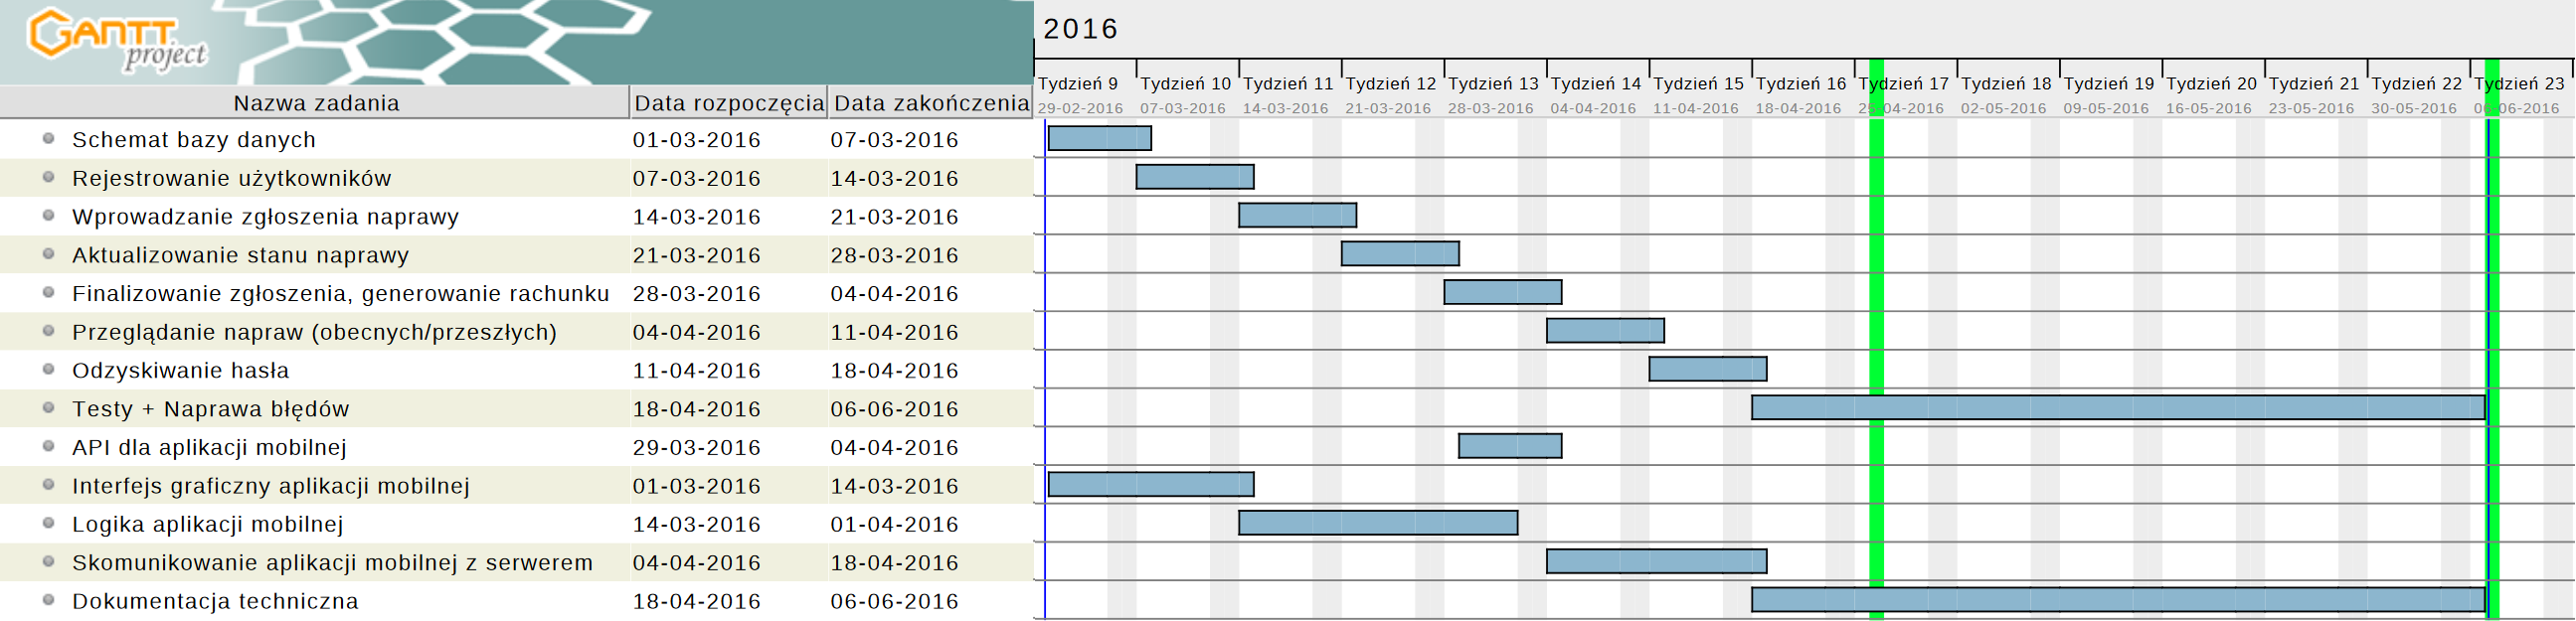
\includegraphics[width=\textwidth,height=0.7\textheight]{gannth1.png}
	\caption{Wykres Gantta - pierwszy kamień milowy}
\end{sidewaysfigure}

Druga wersja diagramu Gantta powstała krótko przed osiągnięciem drugiego kamienia milowego. Został uzupełniony postęp poszczególnych funkcjonalności aplikacji, a do listy zadań dodane zostały wybrane funkcjonalności rozszerzone. Poprawiony diagram znajduje się na rysunku 3.2.
\begin{sidewaysfigure}[h!]
	\centering
	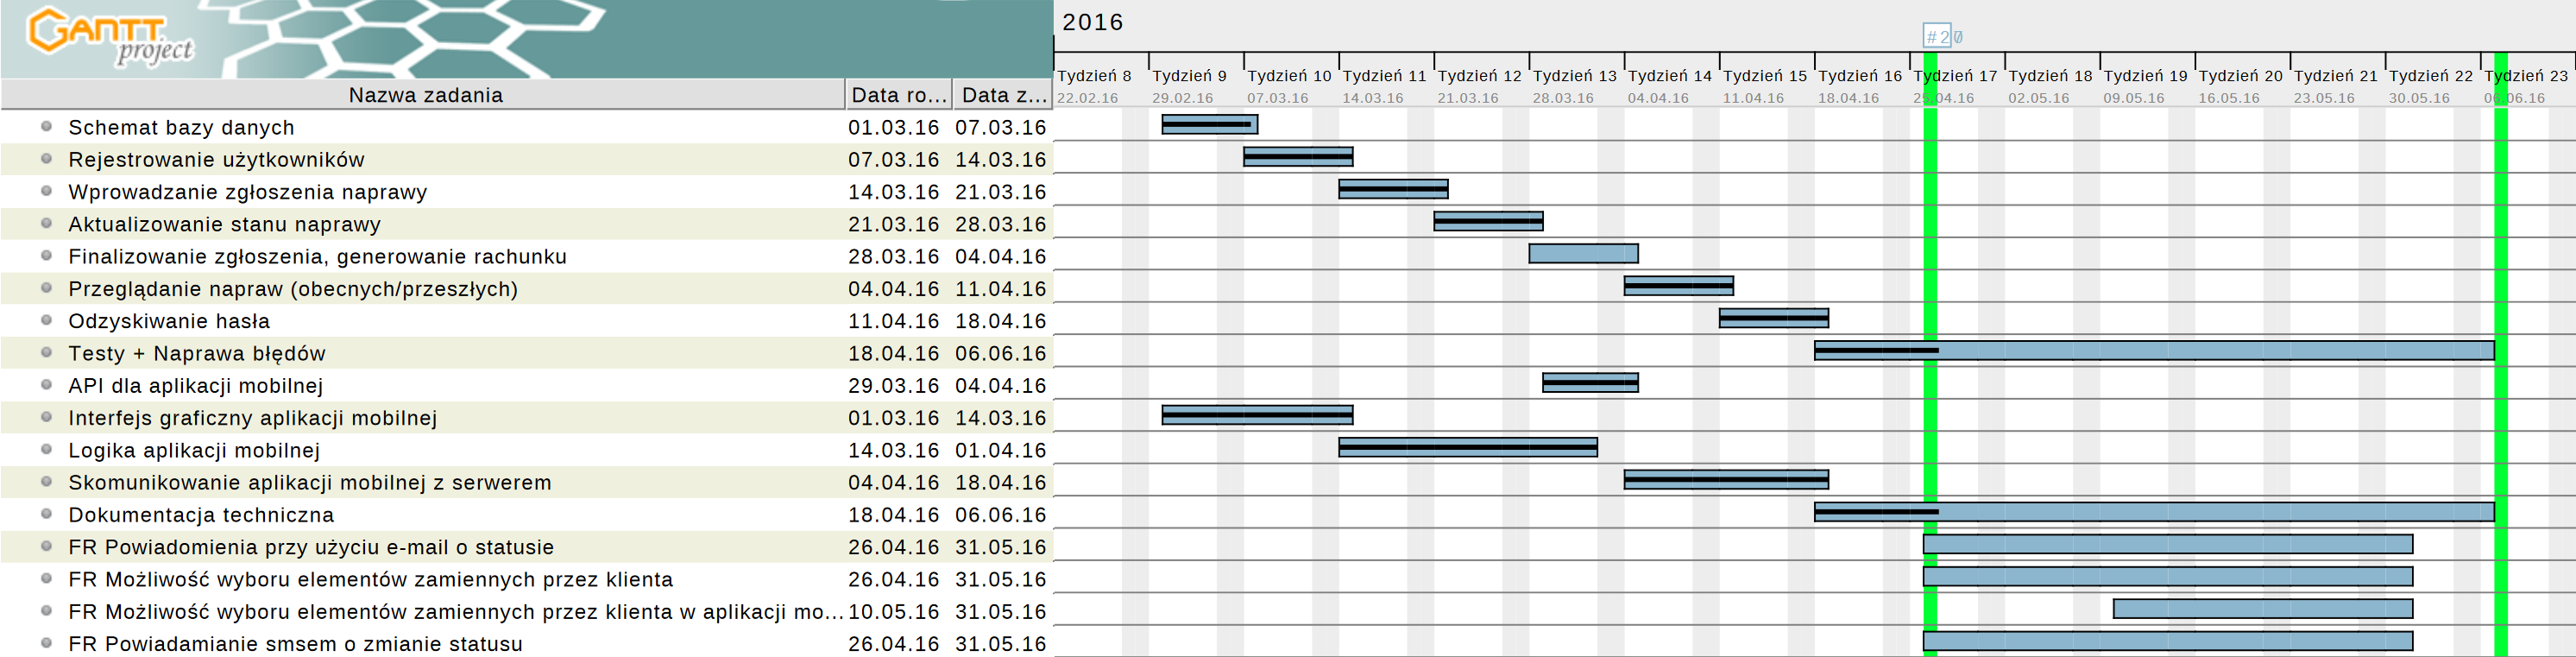
\includegraphics[width=\textwidth,height=0.7\textheight]{gannth2.png}
	\caption{Wykres Gantta - drugi kamień milowy}
\end{sidewaysfigure}

Trzecia wersja diagramu Gantta powstała na sam koniec prac projektowych. Ponownie zaktualizowany został postęp poszczególnych funkcjonalności aplikacji, większość których została już ukończona w 100\%. Finalną wersję diagramu przedstawia rysunek 3.3.
\begin{sidewaysfigure}[h!]
	\centering
	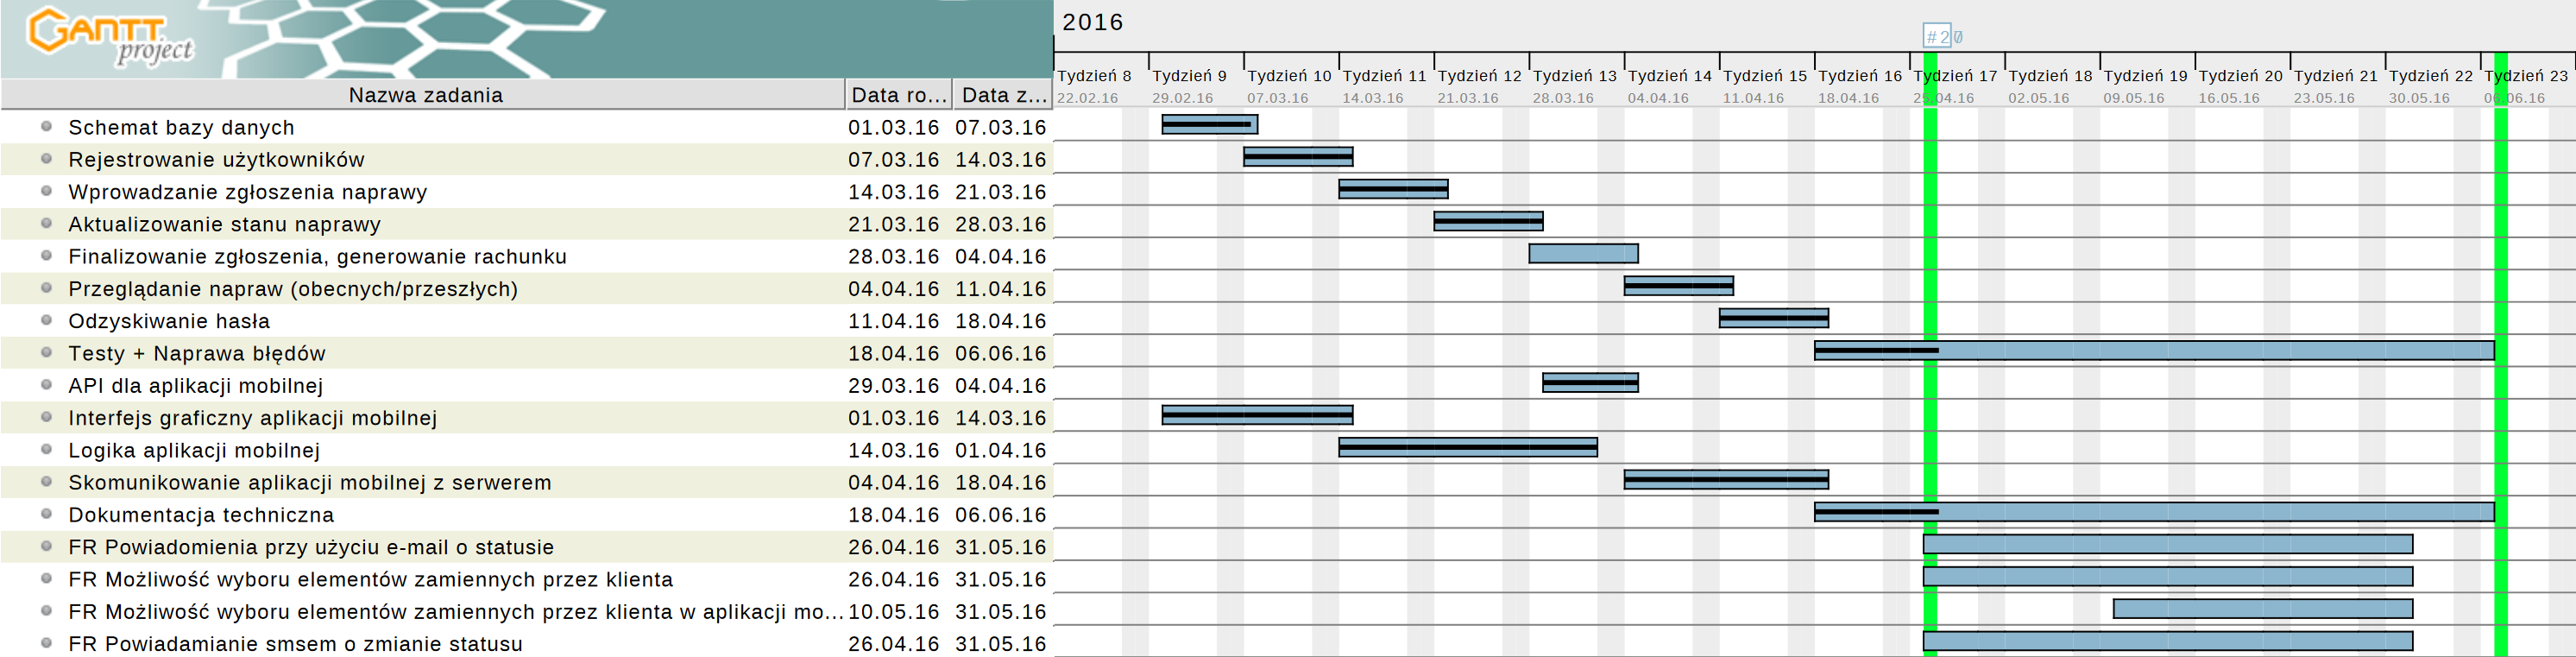
\includegraphics[width=\textwidth,height=0.7\textheight]{gannth3.png}
	\caption{Wykres Gantta - trzeci kamień milowy}
\end{sidewaysfigure}
\subsection{Rzeczywisty nakład pracy i koszty}
Ze względu na otwarty charakter dostarczanego oprogramowania i brak planowanych bezpośrednich zysków z przedsięwzięcia zdecydowano o nieokreśleniu średniej stawki godzinowej pracy członka zespołu w projekcie. Konsekwentnie nie zostały obliczone sumaryczne koszty wytworzenia kompletnego produktu, jedynie nakład pracy wyrażony w godzinach.
Rzeczywisty sumaryczny nakład pracy w projekcie różni się od antycypowanego w znaczącym stopniu ze względu na to, że podczas oryginalnego szacunku pominięto implementację funkcjonalności rozszerzonych aplikacji oraz stworzenie aplikacji mobilnej na urządzenia z systemem Android. Pierwotny plan czasu pracy okazał się jednak być bardzo celny w zakresie funkcjonalności podstawowych systemu. Rzeczywisty czas realizacji poszczególnych funkcjonalności był następujacy (w nawiasach wartości przewidywane):
\begin{itemize}
	\item stworzenie schematu bazy danych - 4h (4h), 
	\item rejestrowanie użytkowników w systemie - 8h (10h), 
	\item wprowadzenie zgłoszenia naprawy - 9h (11h),
	\item aktualizowanie stanu naprawy - 11h (8h),
	\item finalizowanie zgłoszenia wraz z generowaniem rachunku - 8h (9h),
	\item przeglądanie napraw - 8h (9h),
	\item odzyskiwanie hasła - 5h (5h).
	\item powiadomienie o statusie przy użyciu e-mail - 3h (brak predykcji)
	\item powiadomienie o statusie przy użyciu SMS - 12h (brak predykcji)
	\item implementacja aplikacji mobilnej - 35h (brak predykcji)
\end{itemize}
Sumaryczny przewidywany czas realizacji funkcjonalności wyniósł 56h, a rzeczywisty czas realizacji funkcjonalności które zostały uwzględnione w predykcjach był o 3 godziny krótszy (spadek o 5.4 \%). Sumaryczny czas wszystkich prac implementacyjnych wynosi 103h, co daje wzrost względem wartości planowanej o 83.9 \%, jednak należy powtórnie podkreślić że tak duża różnica wynika z nieuwzględnienia prac nad aplikacją mobilną w trakcie pierwotnych predykcji.

\section{Implementacja i wdrożenie projektu}
W ramach realizacji projektu zaimplementowana została wielowarstwowa aplikacja internetowa z rozszerzeniem o aplikację mobilną. Model bazy danych stworzono zgodnie z podejściem „Database First” z wykorzystaniem technologii ADO.NET. Jako narzędzie do mapowania obiektowo relacyjnego wykorzystano platformę Entity Framework, natomiast zapytania do bazy danych zostały napisane w języku LINQ. Warstwa dostępu do danych została odseparowana od logiki aplikacji z wykorzystaniem warstwy logiki biznesowej. Utworzone zostały modele transferu danych odzwierciedlające modele warstwy dostępu do danych oraz modele widoku je zawierające, po to aby uniknąć korzystania z modeli warstwy dostępu do danych w warstwie aplikacji.

Warstwa logiki aplikacji oraz warstwa prezentacji zostały zrealizowane w oparciu o platformę ASP.NET MVC 5. Autentykację użytkowników uzyskano z wykorzystaniem ASP.NET Identity. Do tworzenia widoków aplikacji wykorzystano składnię Razor, a sterowanie aplikacją zrealizowano za pomocą składnika platformy MVC o nazwie HTML Helper; wykorzystano również składniki biblioteki jQuery UI. Od strony wizualnej widoki zostały zaprojektowane z wykorzystaniem biblioteki Bootstrap oraz autorskich stylów CSS.

Dzięki ogromnym możliwościom dostarczonym przez Entity Framework pomimo relatywnie skomplikowanej struktury bazy danych operacje typu CRUD nie przysparzają żadnego problemu. Wielką zaletą stosowanego narzędzia jest fakt, że obiekty bazodanowe zawierają referencje do powiązanych ze sobą tabel, dzięki czemu w bardzo prosty sposób można pobrać z bazy dane z powiązanych ze sobą tabel. Do mapowania obiektów warstwy dostępu do danych na obiekty transferowe wykorzystano Automapper. Podejście takie daje gwarancję że w razie rozbudowy bazy danych wystarczy uzupełnić obiekty warstwy transferu danych o nowe pola, nie trzeba natomiast przejmować się mapowaniem.

Aplikacja mobilna została napisana w języku Android i została zaprojektowana na urządzenia z minimalną wersją systemu operacyjnego 4.0 (Ice Cream Sandwich). Do komunikacji z serwerem wykorzystywane jest własnoręcznie stworzone API bazujące na metodach HTTP POST i GET, a dane są przesyłane w formacie JSON. Aplikacja dzieli się na graficzny interfejs użytkownika (zawarty w plikach xml) oraz część backendową (pliki java). Pierwszym widokiem otwieranym bezpośrednio po uruchomieniu aplikacji jest \texttt{activity\_login.xml}, a klasy i metody tej aktywności zostały zaimplementowane w pliku LoginActivity.java. Wszystkie kolejne aktywności zostały zaimplementowane analogicznie jak w powyższym przykładzie.

Wśród najważniejszych aktywności aplikacji mobilnej należy wyróżnić:
\begin{itemize}
	\item \texttt{activity\_login.xml} - ekran logowania aplikacji  wyświetlający logo aplikacji i pozwalający na zmianę języka,
	\item \texttt{activity\_panel\_components.xml} - wyświetlenie dostępnej listy części zamiennych,
	\item \texttt{activity\_panel\_services.xml} - wyświetlenie listy zgłoszeń użytkownika pokolorowanych w zależności od ich statusu.
\end{itemize}
\subsection{Diagram technologii wykorzystanych w projekcie}
Rysunek 4.1 przedstawia schemat połączeń pomiędzy poszczególnymi komponentami projektu i wykorzystane technologie.
\begin{figure}[H]
	\centering
	\includegraphics[width=\textwidth,height=0.6\textheight]{diagramTechnologii.png}
	\caption{Diagram wykorzystanych technologii}
\end{figure}
\subsection{Instalacja projektu i wymagania sprzętowe}
Ze względu na charakter projektu (open source) fizyczny proces wzdrożenia aplikacji we własnym serwisie napraw leży w gestii właściciela serwisu. Jeśli posiada on własny serwer z bazą danych MS SQL i działającą usługą internetową IIS	wystarczy wykonać wykonać następujące kroki:
\begin{itemize}
	\item folder zawierający stronę internetową umieścić w folderze \texttt{C:\textbackslash inetpub\textbackslash wwwroot},
	\item przejść do \texttt{start -> uruchom -> inetmgr} aby otworzyć okno zarządzania aplikacjami internetowymi i uruchomić serwer (patrz rysunek 4.2).
\end{itemize}
\begin{figure}[h!]
	\centering
	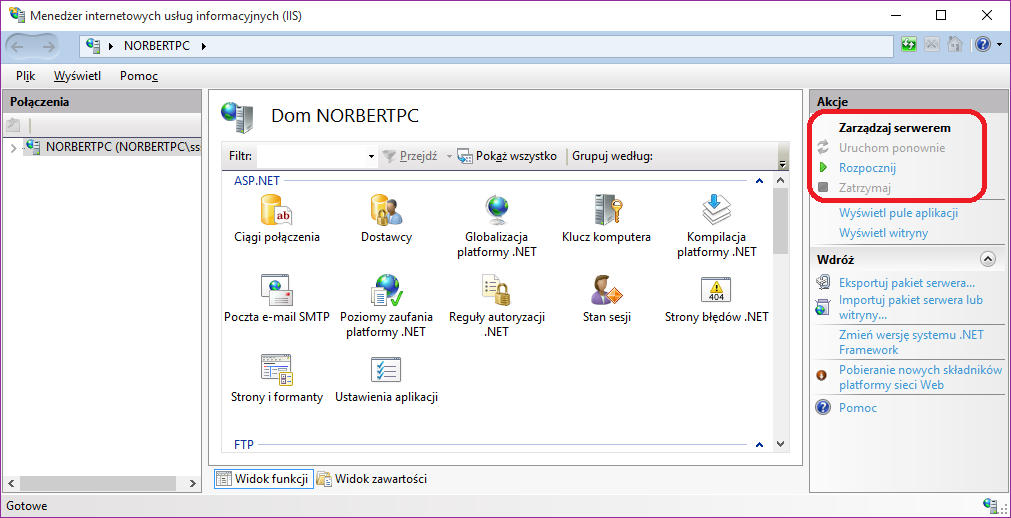
\includegraphics[width=\textwidth,height=0.6\textheight]{inetMgr.png}
	\caption{Ręczne uruchomienie serwera na lokalnej maszynie}
\end{figure}
Jeśli jednak użytkownik nie posiada takiej możliwości zachodzi konieczność wykupienia hostingu. Przykładowym portalem oferującym zarówno serwer usług internetowych IIS jak i serwer bazodanowy MS SQL jest witryna somee.com. Po ukończeniu procesu rejestracji i wykupieniu żądanego przez nas planu usługowego możemy utworzyć swoją stronę internetową, co przedstawiają rysunki 4.3 i 4.4.
\begin{figure}[h!]
	\centering
	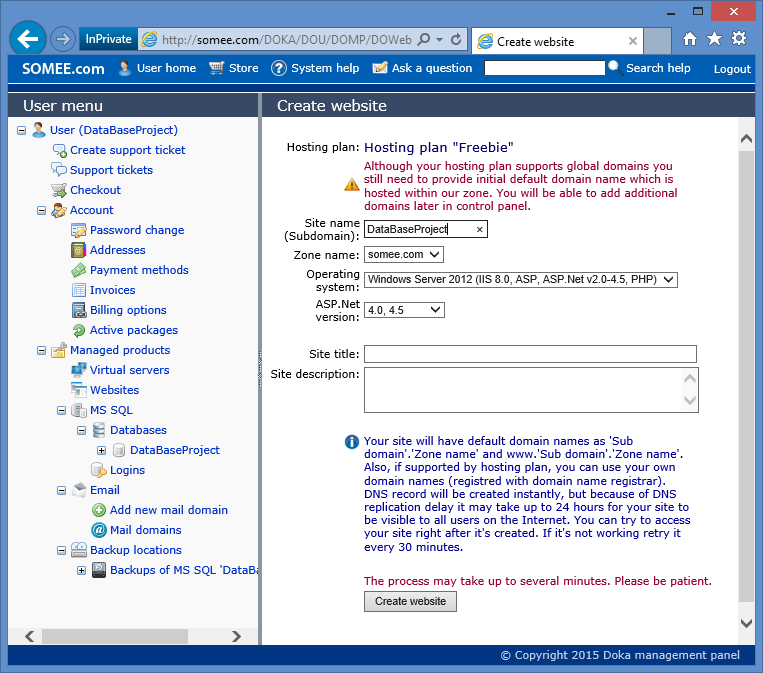
\includegraphics[width=\textwidth,height=0.6\textheight]{somee1.png}
	\caption{Zakładanie strony internetowej cz.1}
\end{figure}
\begin{figure}[h!]
	\centering
	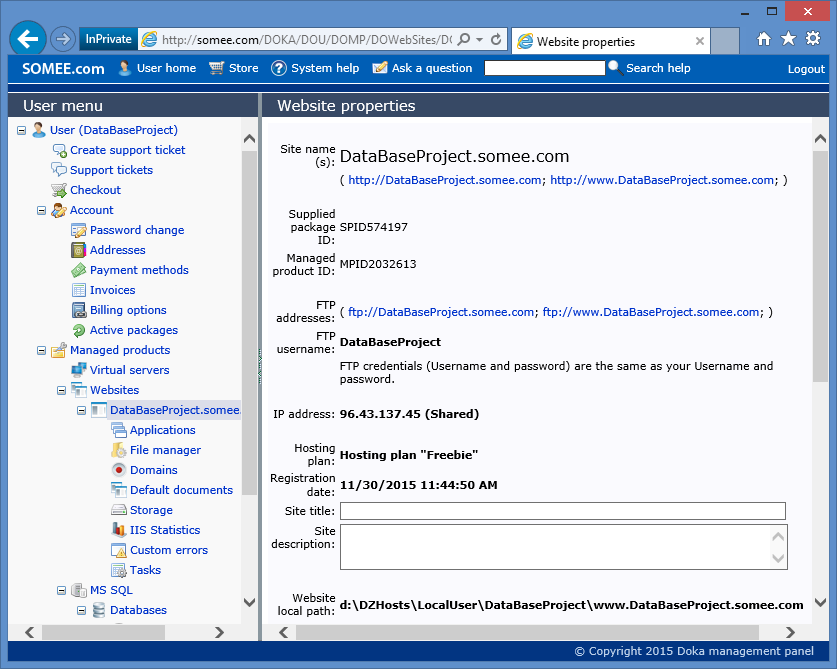
\includegraphics[width=\textwidth,height=0.6\textheight]{somee2.png}
	\caption{Zakładanie strony internetowej cz.2}
\end{figure}
Następnym krokiem jest instalacja naszej aplikacji na zdalnym serwerze. Proces ten znacząco może uprościć IDE Visual Studio, wymagając od użytkownika jedynie kliknięcia opcji \texttt{publish} i wybrania profilu publikacji. Przedstawiają to rysunki 4.5 i 4.6.
\begin{figure}[h!]
	\centering
	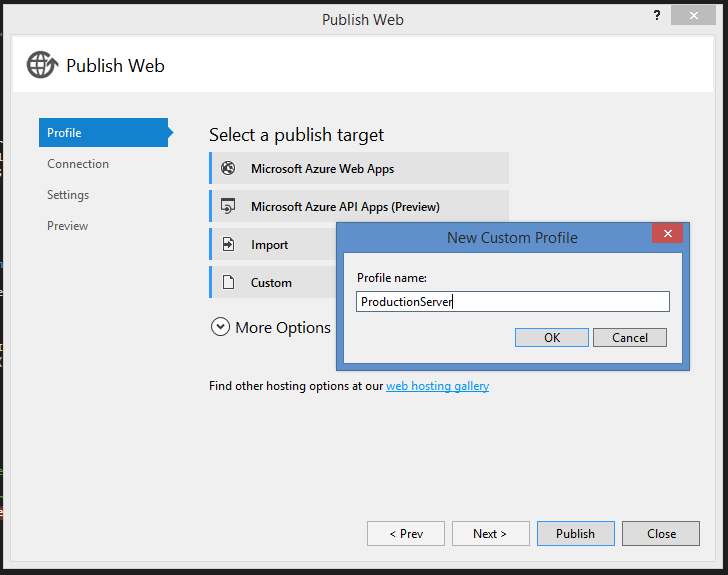
\includegraphics[width=\textwidth,height=0.6\textheight]{vs2.png}
	\caption{Tworzenie profilu}
\end{figure}
\begin{figure}[h!]
	\centering
	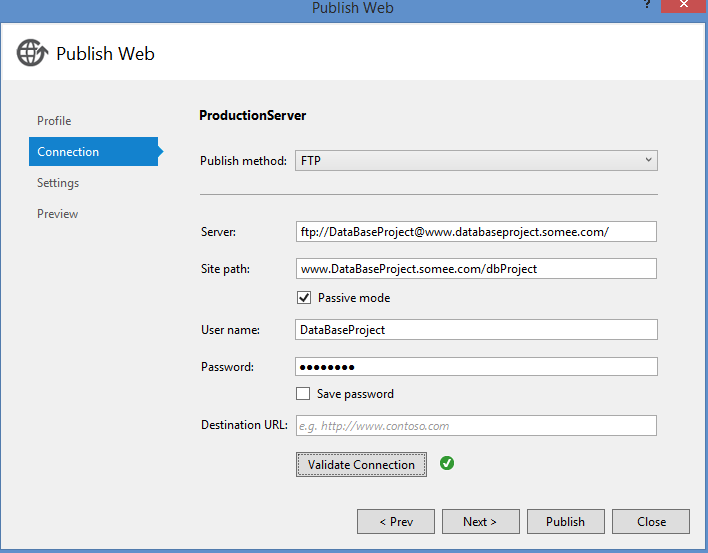
\includegraphics[width=\textwidth,height=0.6\textheight]{vs3.png}
	\caption{Wybór adresu serwera i publikacja projektu}
\end{figure}
Ostatnim brakującym elementem układanki jest połączenie serwera z bazą danych. Analogicznie jak w przypadku samej aplikacji, jeśli nie mamy możliwości umieszczenia jej na własnym serwerze jesteśmy zmuszeni skorzystać z hostingu wykonując proces zbliżony do publikowania samej aplikacji. Dodatkowo aby zapewnić komunikację pomiędzy aplikacją a bazą danych należy zdefiniować odpowiedni connection string w pliku konfiguracyjnym Web.config. Czynności te zostały zaprezentowane na rysunkach od 4.7 do 4.9.
\begin{figure}[h!]
	\centering
	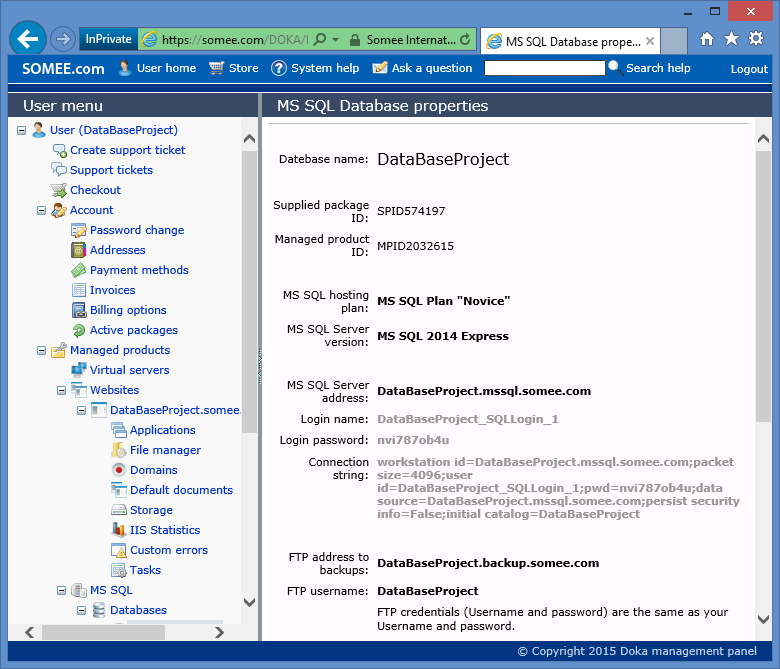
\includegraphics[width=\textwidth,height=0.6\textheight]{db1.png}
	\caption{Hosting bazy danych}
\end{figure}
\begin{figure}[h!]
	\centering
	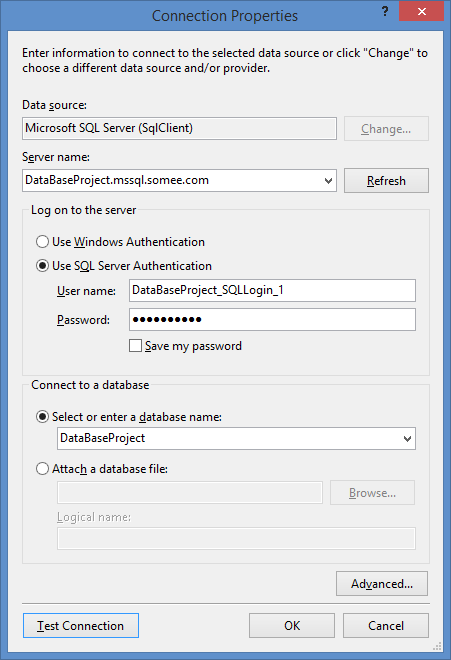
\includegraphics[width=\textwidth,height=0.6\textheight]{db3.png}
	\caption{Ustawienia połączenia}
\end{figure}
\begin{figure}[h!]
	\centering
	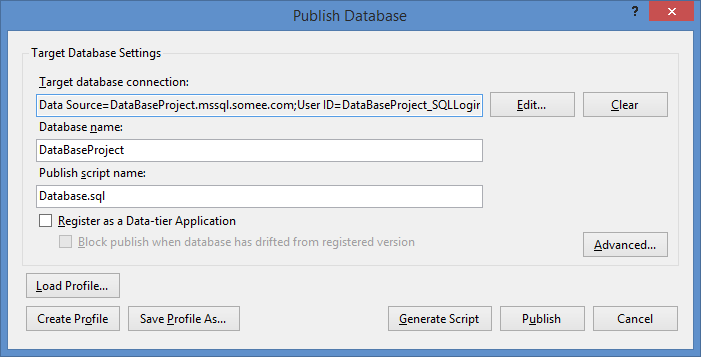
\includegraphics[width=\textwidth,height=0.6\textheight]{db4.png}
	\caption{Publikacja bazy danych}
\end{figure}

Wdrożenie aplikacji mobilnej jest relatywnie prostym procesem. Po umieszczeniu aplikacji webowej na wybranym serwerze należy zmienić wykorzystywany URL w czterech plikach źródłowych aplikacji (\texttt{services\_details.java, panel\_services.java, panel\_components.java i LoginActivity.java}) na adres działającego własnego serwera, a następnie zbudować całą aplikację od początku. Otrzymany plik \texttt{*.apk} możemy już udostępnić do pobrania klientom serwisu np. poprzez istniejącą stronę internetową.
\subsection{Instrukcja obsługi systemu}
\section{Podsumowanie}

\newpage
\listoffigures
\addcontentsline{toc}{section}{Spis rysunków} 
\newpage
\listoftables
\addcontentsline{toc}{section}{Spis tablic}



\newpage
\addcontentsline{toc}{section}{Literatura}
\begin{thebibliography}{9}
\bibitem{cormen} Cormen T., Leiseron C., Rivest R., Wprowadzenie do algorytmów, WNT, 2001. 
\bibitem{kombi} Błażewicz J., Problemy optymalizacji kombinatorycznej, PWN, Warszawa, 1996.
\bibitem{tabu} Strona internetowa: http://www.cs.put.poznan.pl/wkotlowski/teaching/8-ts.pdf, 25.01.2013r.
\end{thebibliography}

\end{document}